\chapter{Stato dell'arte}
\label{chap:SOA}
\vspace{1cm}
In questo capitolo verrà fornito un esame dello stato dell'arte e verranno presentate 
alcune soluzioni relative al lavoro oggetto di questa tesi.

Nella Sezione \ref{sec:progettoFASTER} è descritto il progetto europeo 
\acs{FASTER} con una spiegazione sulla metodologia proposta per la toolchain e 
l'algoritmo che effettua l'analisi esplorativa delle soluzioni, che interagisce 
con lo scheduler.

Nella Sezione \ref{sec:algoritmiProposti} si esaminano i vari approcci proposti 
dagli autori nell'ambito del problema dello scheduling dei task su dispositivi 
riconfigurabili, divisi in algoritmi esatti, trattati nella Sezione 
\ref{sec:algoritmiEsatti}, ed euristici, trattati nella Sezione 
\ref{sec:algoritmiEuristici}.


\section[Il progetto \acs{FASTER}]{Il progetto \acs{FASTER}}
\label{sec:progettoFASTER}
In questa sezione vengono presentate il fondamento logico e le motivazioni alla 
base del progetto \acs{FASTER}. La Sezione \ref{sec:fasterIntro} fornisce 
un'introduzione al progetto e spiega gli obiettivi e le motivazioni alla 
base che hanno portato alla creazione del progetto; infine, la Sezione 
\ref{sec:fasterMetodologia} illustra la metodologia tramite la quale si possono 
raggiungere gli obiettivi prefissati.


%%% acro definitions
\acrodef{NIDS}{Network Intrusion Detection System}
\acrodef{RTM}{Reverse Time Migration}
\acrodef{TCO}{Total Cost of Ownership}
\acrodef{ICS}{Institute of Computer Science}
\acrodef{FORTH}{Foundation for Research and Technology - Hellas}
%%%%%%%%%%%%%%%%%%%%%%%%%%%%%%%%%%%%%%


\subsection{Introduzione}
\label{sec:fasterIntro}
\acs{FASTER} è l'acronimo di \emph{\acl{FASTER}}, un progetto\footnote{Sito del 
progetto: \url{http://www.fp7-faster.eu/}.} organizzato dalla comunità europea 
che coinvolge diverse aziende e atenei\footnote{I collaboratori del progetto 
sono: l'\ac{ICS} di \ac{FORTH} in Grecia, Chalmers University of Technology in 
Svezia, l'università di Ghent in Belgio, l'Imperial College di Londra, il 
Politecnico di Milano e le aziende Maxeler, ST Microelectronics e Synelixis.}, 
tra cui il Politecnico di Milano. Il progetto è stato avviato il 1 settembre 
2011, ha una durata di 36 mesi ed è supportato tramite fondi stanziati dalla 
comunità europea.

\subsubsection{Motivazioni e obiettivi del progetto}
L'ambito di applicazione del progetto \ac{FASTER} sono le architetture 
riconfigurabili; in particolare, \ac{FASTER} è pensato, come il nome 
suggerisce, per facilitare la definizione e l'uso di sistemi implementati in 
hardware \cite{FasterPaper}.

Sfruttando le potenzialità delle promettenti architetture hardware basate sulla 
logica riconfigurabile, introdotte nel Capitolo \ref{chap:intro}, si possono 
infatti estendere le funzionalità (e quindi la durata della vita) di 
un'applicazione senza dover riprogettare interamente l'hardware necessario per 
eseguirla, consentendo allo stesso tempo di raggiungere performance equiparabili 
a quelle di un'esecuzione su hardware dedicato.

% FIXME spostare nell'introduzione?
Si pensi, a titolo esemplificativo, a un \ac{NIDS}, il cui scopo è eseguire la 
scansione di tutti i pacchetti in ingresso per rilevare possibili minacce, e 
tale scansione deve essere sufficientemente veloce da non costituire un collo 
di bottiglia e rallentare così le comunicazioni. Inoltre, nuove regole devono 
essere aggiunte costantemente, con il crescere della lista delle minacce. In 
risposta a questi requisiti di velocità e dinamicità dell'applicazione, la 
logica riconfigurabile rappresenta una soluzione per il soddisfacimento di 
entrambi i requisiti.

% Extending product functionality and lifetime requires constant addition of new 
% features to satisfy the growing customer needs and the evolving market and 
% technology trends. Software component adaptivity is straightforward but not 
% enough: recent products include hardware accelerators - for reasons of 
% performance and power efficiency - that also need to adapt to new 
% requirements.For example, a Network Intrusion Detection System (NIDS) needs to 
% scan all incoming network packets for suspicious content. The scanning has to be 
% fast so that the monitored communication links are not slowed down, while the 
% list of threats to check for is extended and updated on a daily basis.
% 
% Reconfigurable logic allows the definition of new functions to be implemented in 
% dynamically instantiated hardware units, combining adaptivity with hardware 
% speed and efficiency. For the Intrusion Detection System example, new rules can 
% be hardcoded into the reconfigurable logic, achieving high performance, while 
% providing the necessary adaptivity to new threats.


Nonostante il vantaggio di utilizzare architetture riconfigurabili rispetto 
all'eseguire le applicazioni puramente in software, il design e 
l'implementazione di un sistema basato su logica riconfigurabile hanno delle 
limitazioni rispetto alla più facile estensione delle funzionalità di 
un'applicazione software, per le seguenti ragioni:
\begin{itemize}
 \item il supporto di tool esterni per il design del sistema è ancora 
``elementare'';
 \item le riconfigurazioni hanno un grande impatto in termini di overhead sul 
tempo di esecuzione dell'applicazione, pertanto devono essere utilizzate con 
attenzione;
 \item la gestione delle risorse disponibili sulla scheda (anche a run-time) è 
interamente affidata all'utente.
\end{itemize}
Oltre a queste limitazioni, il designer ha altri compiti da assolvere per 
implementare correttamente un sistema su hardware riconfigurabile, tra cui 
l'identificazione di quali parti del codice devono essere eseguite in hardware 
per avere un effettivo guadagno in termini di velocità di esecuzione, quali 
moduli hardware possono beneficiare di una riconfigurazione, stabilire uno 
schedule e verificare la bontà della soluzione così ottenuta.

Il progetto \ac{FASTER} concentra dunque i propri obiettivi nell'introduzione 
di una nuova metodologia che permetta ai designer di implementare facilmente un 
sistema su una piattaforma target dotata di processori general-purpose e 
acceleratori hardware basati su logica riconfigurabile. Questa metodologia 
consentirà, partendo da un input costituito da una descrizione ad alto livello 
sia dell'applicazione che dell'architettura, di sfruttare al massimo le 
possibilità offerte dalla riconfigurazione parziale dinamica.

\paragraph{Lavori precedenti}
Tra i lavori di ricerca e progetti europei più relativi a \ac{FASTER} si 
annoverano \emph{hArtes} \cite{HArtes}, \emph{Morpheus}, \emph{ACOTES} 
\cite{AcotesUrl, ACOTES}, \emph{Andres} e \emph{Reflect} \cite{Reflect}. % 
% FIXME citazioni mancanti perchè i siti sono offline
Questi lavori hanno obiettivi simili a quelli di \ac{FASTER}, tuttavia si 
concentrano più sugli aspetti architetturali della riconfigurazione; in questi 
lavori non si accenna esplicitamente al design della riconfigurazione parziale 
dinamica, nè si considera quale granularità è meglio utilizzare per la 
riconfigurazione: \emph{region-based}\footnote{Nella riconfigurazione di tipo 
region-based, sono riconfigurati interi moduli che occupano arbitrarie porzioni 
della scheda.} oppure \emph{micro-riconfigurazione}\footnote{Nella 
micro-riconfigurazione vengono identificati dei parametri del modulo che 
sono soggetti a cambiamenti; tali parametri non vengono inclusi nel bitstream, 
lasciando così dei ``buchi''. Quando i valori per tali parametri devono essere 
fissati, è sufficiente lanciare una riconfigurazione con un bitstream di 
dimensioni molto ridotte, che vada a modificare solamente i buchi lasciati in 
precedenza.}.

\paragraph{Contributi di \ac{FASTER}}
\ac{FASTER} si distingue rispetto ai lavori precedentemente sviluppati in 
quanto ha come obiettivo l'introduzione della riconfigurazione parziale 
dinamica come un concetto di design esplicito, fornendo anche i metodi per 
supportare la riconfigurazione a run-time nell'intera metodologia di design.
Il progetto \ac{FASTER}, quindi, deve possedere le seguenti caratteristiche:
\begin{enumerate}
 \item deve fornire supporto per l'inclusione della riconfigurazione parziale 
dinamica, sia region-based che micro-riconfigurazione, in maniera trasparente 
all'utente;
 \item deve fornire un framework per il design di un sistema su logica 
riconfigurabile, gestendo l'analisi, la sintesi e la verifica delle soluzioni 
ottenute.
\end{enumerate}

% TODO da scrivere meglio
Gli obiettivi che il progetto \ac{FASTER} si prefigge di raggiungere sono un 
significativo aumento della produttività nel design e nell'implementazione di 
sistemi riconfigurabili, aumento delle performance delle applicazioni 
sviluppate in hardware in presenza di vincoli sul consumo energetico e 
riduzione del costo totale di proprietà\footnote{In inglese \emph{\ac{TCO}}, 
rappresenta l'insieme di tutti i costi da sostenere per l'intero ciclo di 
vita di un sistema o un'apparecchiatura IT.} per sistemi come \ac{NIDS} e 
\ac{RTM} implementati su hardware riconfigurabile, grazie alla minore 
manutenzione richiesta.

Nella prossima sezione verranno illustrate le piattaforme hardware supportate 
da \ac{FASTER} e la metodologia proposta per il framework.


% We expect that the 
% project will lead to a 20% productivity improvement due to seamless 
% implementation and verification of dynamically changing systems, a 50% total 
% ownership cost reduction for NIDS and Reverse Time Migration systems, with a 2x 
% performance improvement under power constraints for Global Illumination and 
% Image Analysis. 


\subsection{Metodologia utilizzata}
\label{sec:fasterMetodologia}

\subsubsection{Piattaforme supportate e applicazioni}
L'obiettivo di \ac{FASTER} è sfruttare le opportunità offerte dalle 
architetture riconfigurabili, sia nel campo dei sistemi \ac{HPC} sia nei 
sistemi embedded. Pertanto, \ac{FASTER} supporta due tipi di piattaforme 
hardware:
\begin{enumerate}
 \item sistemi \ac{HPC} desktop, ad esempio \emph{Maxeler MaxWorkstation};% TODO
 \item sistemi embedded basati su \ac{FPGA}, ad esempio la 
scheda \emph{University Program XUPV5-LX110T} di \emph{Xilinx} o la scheda 
\emph{ZedBoard} di \emph{AVNET}.
\end{enumerate}

Oltre a supportare queste differenti piattaforme, \ac{FASTER} ha come obiettivo 
l'aumento delle performance di tre applicazioni provenienti da diversi ambiti:
\begin{itemize}
 \item \acf{RTM}, un algoritmo applicato nella tomografia sismica per 
fornire una rappresentazione più realistica del sottosuolo in aree 
geologicamente complesse e caratterizzate da differenti velocità di 
propagazione delle onde sismiche;
 \item Global Illumination and Image Analysis, un insieme di algoritmi 
utilizzati per rendere più realistici oggetti e scene rappresentati in grafica 
computerizzata tridimensionale;
 \item sistemi di riconoscimento di intrusione in una rete, descritti in 
precedenza;
\end{itemize}

\subsubsection{Descrizione del framework}
In questa sezione viene descritto il framework e il flusso del progetto ad  
alto livello.

%%% FIXME credit to Santa?
\begin{figure}
 \begin{center}  
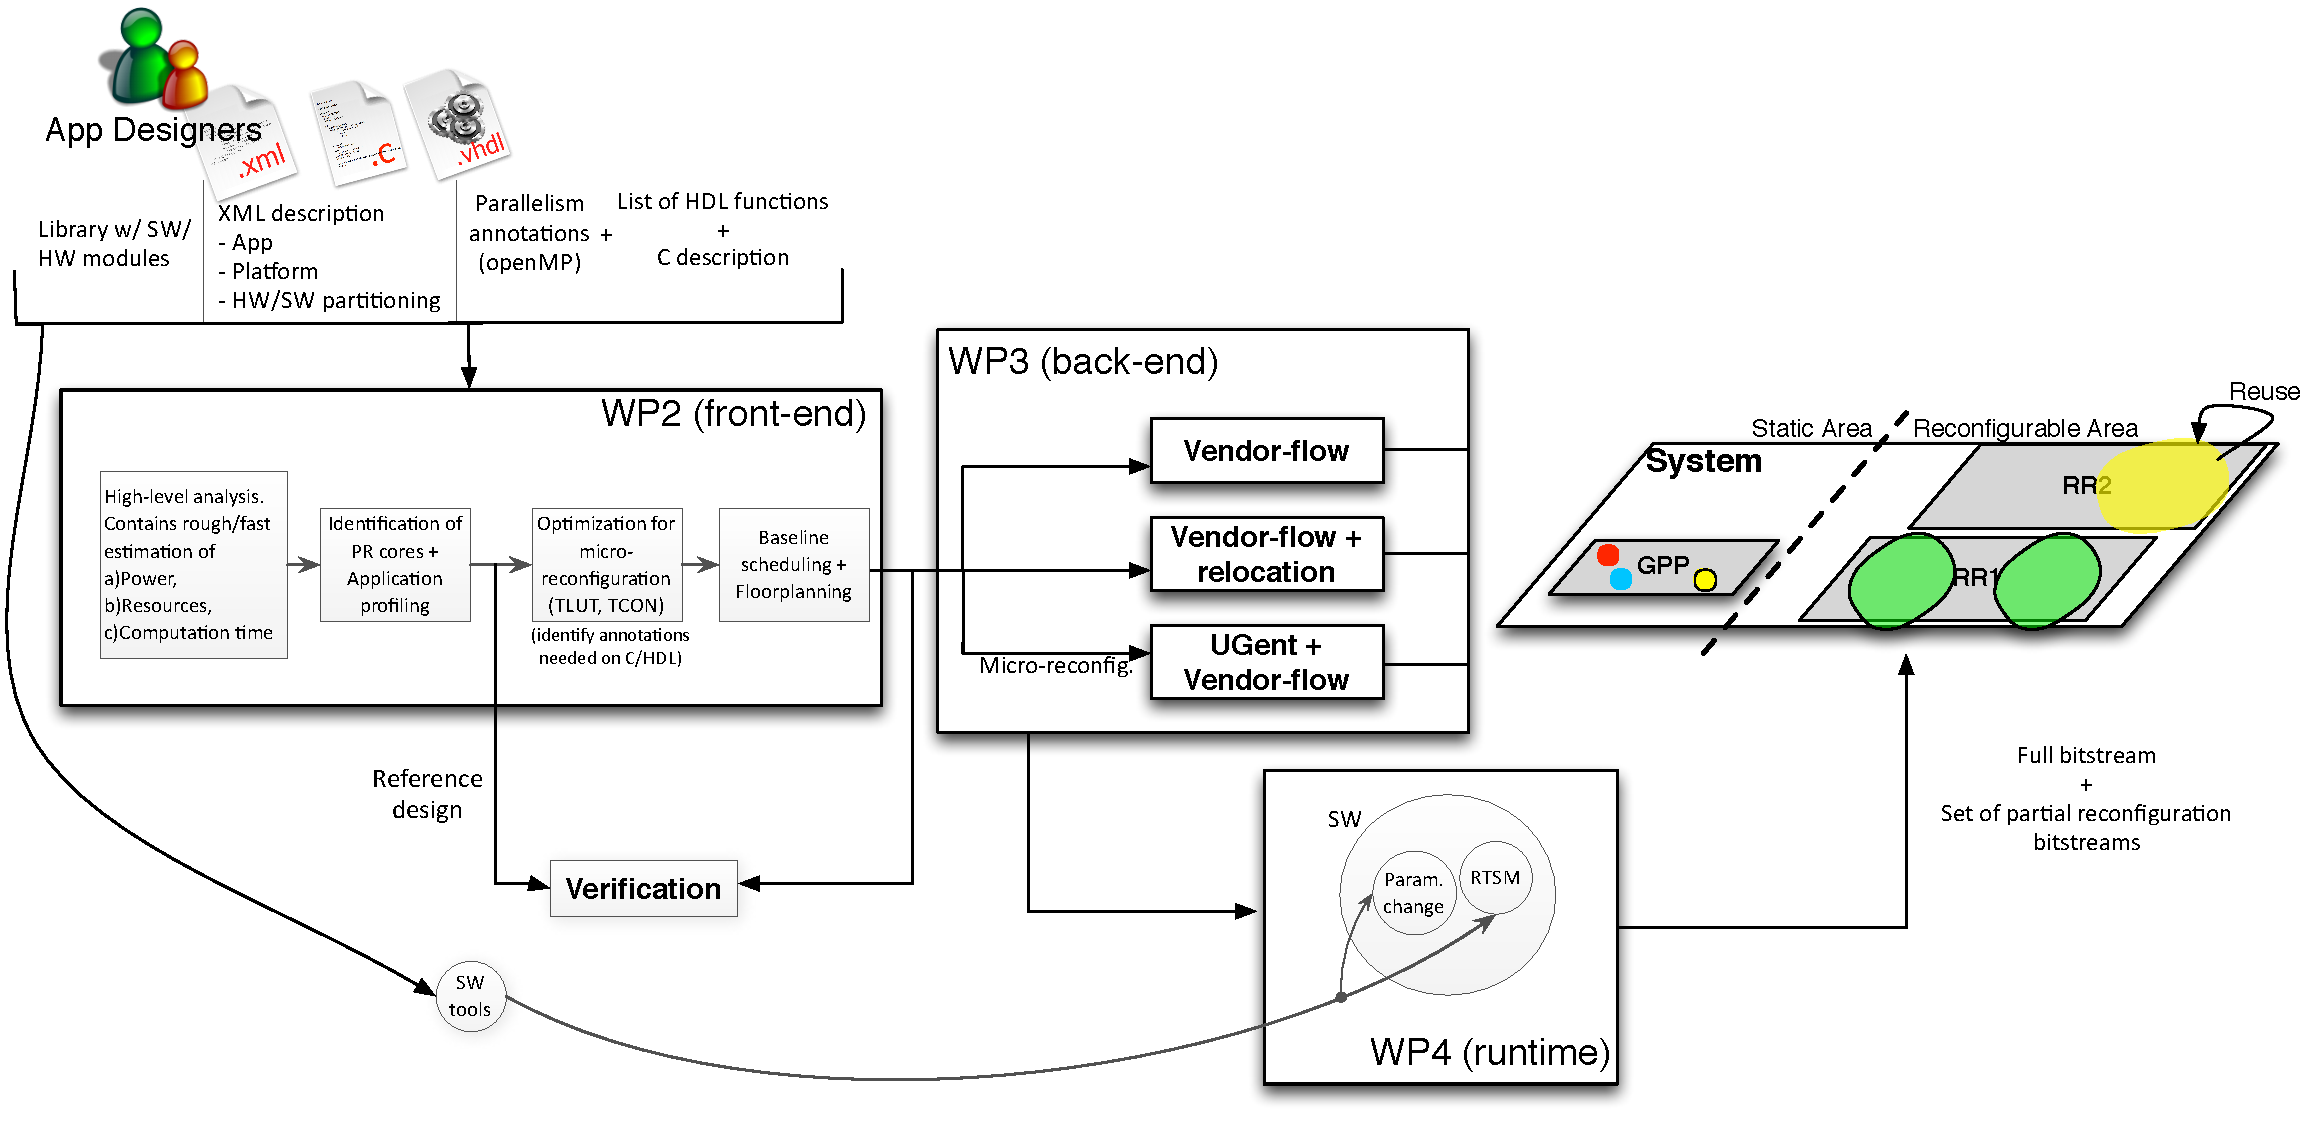
\includegraphics[width=0.9\textwidth]
{capitoli/figure/cap2/FASTERWorkflow.pdf}
\caption{Workflow di \ac{FASTER}.}
\label{fig:FASTERWorkflow}
 \end{center}
\end{figure}

La Figura \ref{fig:FASTERWorkflow} illustra la panoramica della metodologia 
adottata da \ac{FASTER} e il flusso di lavoro che, partendo dalla specifica 
dell'applicazione annotata e dalla descrizione dell'architettura target, riesce 
a derivare un bitfile utilizzabile per configurare l'architettura ed eseguire 
l'applicazione tramite un runtime manager.

L'approccio adottato da \ac{FASTER} prevede che i vari componenti del framework 
si interfaccino tra loro mediante l'uso di file XML. L'input di un progetto 
\ac{FASTER} è costituito dall'applicazione da sintetizzare, che può 
essere scritta in un linguaggio ad alto livello (ad esempio, il linguaggio C) e 
provvista di annotazioni, ad esempio in formato OpenMP\footnote{OpenMP è un 
formato standard per la specifica di applicazioni parallele, che permette di 
specificare quali funzioni di un'applicazione sono parallelizzabili e di 
suddividere l'applicazione nei vari task.}, che ne consentono la suddivisione 
iniziale in task e dalla descrizione delle funzionalità di riconfigurazione a 
disposizione dell'architettura. Oltre all'applicazione possono essere presenti 
degli attributi specificati dal designer che impongono vincoli particolari 
all'applicazione, quali ad esempio scadenze nell'esecuzione oppure una 
richiesta in termini di throughput.

\paragraph{High-level analysis}
La prima fase del flusso di lavoro prevede l'analisi ad alto livello 
dell'applicazione e dei suoi requisiti. In questa fase è fornito un modello di 
design riconfigurabile che mette in relazione i requisiti dell'applicazione con 
determinate metriche di valutazione delle performance.

Tramite questo processo si possono identificare dei componenti e determinare le 
performance delle relative implementazioni: esempi di parametri relativi ad 
un'implementazione sono le stime di risorse occupate, dell'overhead introdotto 
dalle riconfigurazioni o del consumo di energia in base all'area occupata su 
scheda.

\paragraph{Identificazione dei core}
Durante questa fase viene analizzata l'applicazione per estrarne i vari core, 
ovvero moduli composti da una serie di operazioni. I moduli sono estratti 
partendo dal \ac{CDFG} dell'applicazione, cercando di identificare opportuni 
sottografi isomorfi; nel caso l'identificazione abbia successo, è possibile 
riutilizzare uno o più moduli senza fare uso di riconfigurazione e guadagnando 
quindi in termini di tempo di esecuzione.
I core possono essere di due tipi:
\begin{enumerate}
 \item \emph{statici}, moduli configurati staticamente e non riconfigurabili 
durante l'esecuzione;
 \item \emph{riconfigurabili}, i quali a loro volta si dividono in:
  \begin{itemize}
   \item \emph{region-based}, in cui l'intero modulo viene riconfigurato;
   \item \emph{micro-riconfigurabili}, in cui solo piccole parti del modulo 
sono riconfigurate e il resto viene riutilizzato.
  \end{itemize}
\end{enumerate}

Al termine dell'identificazione dei core, si svolge la fase di 
\emph{partitioning}, in cui si stabilisce quali parti dell'applicazione debbano 
essere eseguite in software su un processore general-purpose e quali in 
hardware su logica riconfigurabile.

\paragraph{Baseline scheduling}
A questo punto, partendo dalle informazioni calcolate nei passi precedenti, 
viene calcolato un baseline schedule dei task sulla piattaforma target. Lo 
schedule viene calcolato da uno scheduler euristico che deve essere conscio 
delle riconfigurazioni che vengono introdotte. Lo scheduler deve quindi 
avere le seguenti funzionalità:
\begin{itemize}
 \item \emph{configuration prefetching}: una riconfigurazione per un 
modulo viene eseguita il prima possibile rispetto all'inizio dell'esecuzione 
del modulo, così facendo in alcuni casi è possibile mascherare l'overhead di 
riconfigurazione;
 \item \emph{riutilizzo dei moduli}: eventuali moduli che devono 
essere eseguiti in hardware (stabilito nella fase di partitioning) e sono 
caratterizzati dalla stessa implementazione non necessitano di riconfigurazione 
dell'area.
\end{itemize}
Obiettivo di questa fase è ottenere uno scheduling \emph{feasible} che abbia il 
minore makespan possibile, non necessariamente il minimo assoluto.

Il floorplanner viene eseguito in questa fase e si occupa del piazzamento dei 
moduli sull'area della scheda \ac{FPGA}; vengono definiti i vincoli spaziali e 
la dimensione delle aree su cui configurare i moduli da eseguire, e viene 
stabilito se un determinato piazzamento è fattibile oppure viola alcuni vincoli.

\paragraph{Generazione del codice} % TODO sistemare e ampliare
In questa fase viene generato il codice necessario per eseguire l'applicazione 
sulla piattaforma target, tramite l'utilizzo di backend specifici per ogni tipo 
di piattaforma supportata.

Partendo dal progetto \ac{FASTER} così creato si può derivare un progetto 
interfacciato con i vari tool sviluppati dal fornitore della piattaforma target 
per la sintesi dei vari IP core o del sistema di comunicazione tra i moduli.


\subsubsection{Conclusioni}
In questa sezione si è fornita una descrizione del progetto europeo 
\ac{FASTER}. Sono state descritte le motivazioni e il fondamento logico alla 
base del progetto, gli obiettivi che esso si profigge di raggiungere nel 
facilitare il design di applicazioni per dispositivi in grado di sfruttare le 
potenzialità offerte dalla \emph{riconfigurazione}. Infine, è stato esaminato 
ad alto livello il flusso di lavoro del progetto e le varie fasi in cui questo 
si divide sono state descritte brevemente.

Nella prossima sezione ci si concentrerà sul lavoro oggetto di questa tesi, 
ovvero la fase di baseline scheduling del progetto; verranno presentate alcune 
soluzioni presenti nello stato dell'arte riguardanti questo problema, con 
relativi pregi e difetti di ognuna.


\section{Algoritmi proposti}
\label{sec:algoritmiProposti}
In questa sezione verranno esaminate diverse soluzioni al problema dello 
scheduling, proposte in altri lavori.

Come anticipato nel Capitolo \ref{chap:intro}, il problema di trovare uno 
schedule di lunghezza minima per un insieme di task in presenza di vincoli di 
risorse appartiene alla classe dei problemi di ottimizzazione 
$\mathcal{NP}$-difficili. Tutte le soluzioni proposte appartengono a una 
tra queste categorie di algoritmi:
\begin{enumerate}
 \item \emph{algoritmi esatti} o \emph{ottimi}, che permettono di ricavare la 
soluzione ottima, tramite l'impiego di opportune strutture matematiche o di 
formulazioni particolari del problema;
 \item \emph{algoritmi euristici}, che in generale portano ad ottenere 
soluzioni subottime. Gli algoritmi euristici si possono suddividere a loro 
volta in sottocategorie in base al loro funzionamento, tra le più importanti 
ricordiamo:
 \begin{itemize}
  \item euristiche basate su una lista, in cui i task vengono schedulati 
secondo l'ordine in cui compaiono nella lista ordinata per priorità decrescenti;
  \item meta-euristiche, che comprendono algoritmi evolutivi o ispirati al 
comportamento di sistemi presenti in natura.
 \end{itemize}
\end{enumerate}

\begin{figure}
 \begin{center}
  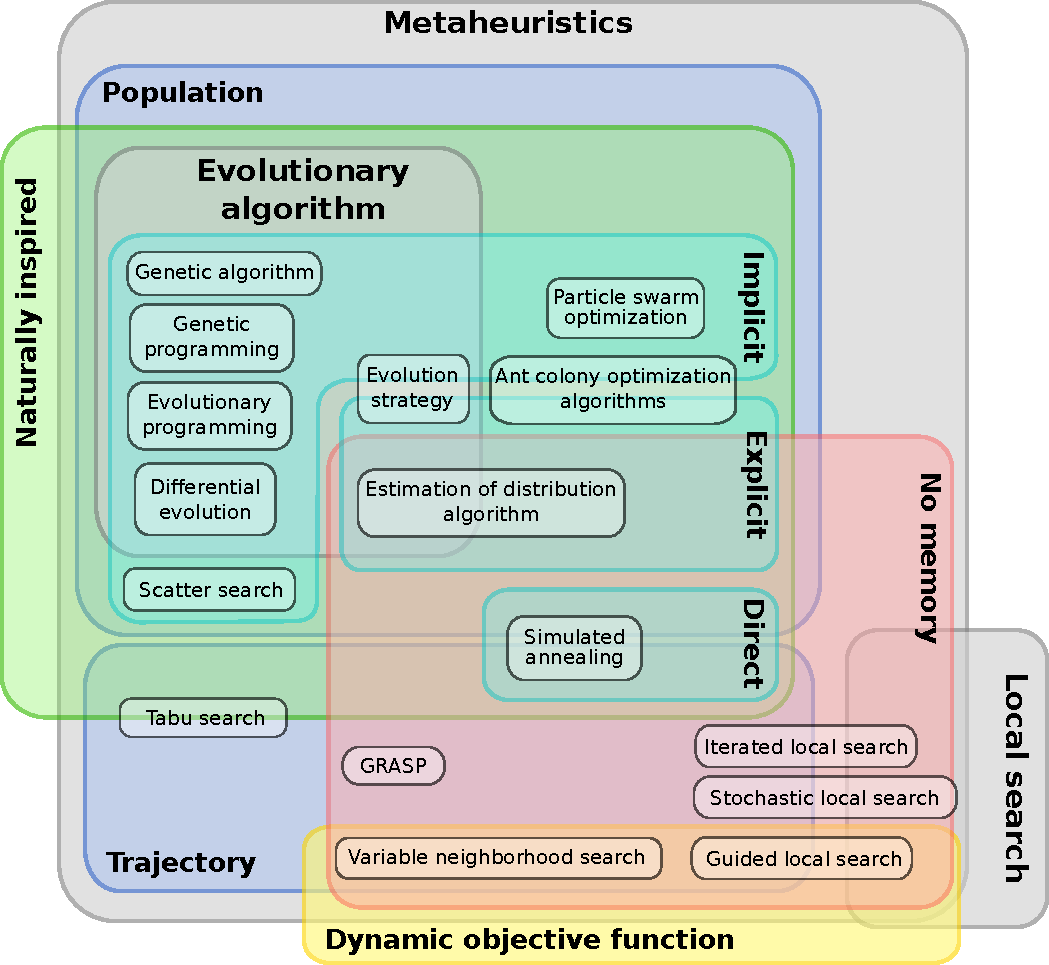
\includegraphics[width=0.7\textwidth]
  {capitoli/figure/cap2/MetaheuristicsClassification.pdf}
  \caption{Classificazione delle varie categorie di meta-euristiche. Immagine 
realizzata da Johann Dréo e tradotta in inglese da Caner Candan.}
\label{fig:metaheuristicsClassification}
 \end{center}
\end{figure}

%%%%%%%%%%
\acrodef{SCOP}{Stochastic Combinatorial Optimization Problem}
%%%%%%%%%%

La classificazione dei diversi tipi di algoritmi meta-euristici è illustrata in 
Figura \ref{fig:metaheuristicsClassification}. Diversi lavori forniscono 
un'analisi di questo tipo di algoritmi euristici, ad esempio lo studio condotto 
da Bianchi et al. \cite{SurveyMetaheuristicSCOP} analizza l'impiego delle 
meta-euristiche per la risoluzione di \acp{SCOP} o l'analisi effettuata da Blum 
et al. \cite{MetaheuristicCombinatorialOptimization} per problemi di 
ottimizzazione combinatoria.

Il resto della sezione è organizzato come segue: nella Sezione 
\ref{sec:algoritmiEsatti} vengono descritte le soluzioni proposte per il 
problema dello scheduling basate su algoritmi esatti; la Sezione 
\ref{sec:algoritmiEuristici} presenta invece le soluzioni basate su metodi 
euristici.


\subsection{Algoritmi esatti}
\label{sec:algoritmiEsatti}
Come esposto nell'introduzione a questa sezione, gli algoritmi esatti 
permettono di ottenere la soluzione ottima in assoluto. Un algoritmo esatto, 
applicato a un problema di ottimizzazione combinatoria qual è un \ac{RCSP}, 
permette di ottenere lo schedule caratterizzato dal minimo makespan possibile. 

A prescindere dal particolare algoritmo utilizzato per risolvere il problema, 
il costo computazionale necessario per giungere a una soluzione è elevato e 
solitamente non polinomiale.


\subsection{Algoritmi euristici}
\label{sec:algoritmiEuristici}


% TODO presentazione delle motivazioni che hanno portato allo sviluppo di un 
% algoritmo iterativo basato su una lista e non esplorativo

% Il flusso di esecuzione della toolchain prevede l'invocazione del tool di 
% scheduling statico come componente esterno da parte dell'algoritmo di 
% esplorazione dello spazio di design del sistema, per la valutazione di una 
% particolare metrica, la stima del tempo di esecuzione totale dello schedule 
% dato un determinato mapping. Poichè la fase di mapping è implementata sotto 
% forma di un  